\chapter{Finite Element Neutron Diffusion}
\label{ch:neutronDiffusion}

\section{Introduction}
  This chapter will describe the solution of the multigroup neutron diffusion 
  equations for general geometry via the \gls{fem}. The solution method and 
  derivations here are general to the multigroup neutron diffusion equation and 
  it's application to fast reactors or any standard reactor geometry is 
  straightforward. For typical fast reactor applications, diffusion theory 
  approximates the neutron distribution within the reactor well. The diffusion 
  approximation is a standard assumption for fast reactors because neutron 
  mean-free-paths within the reactor are large relative to material dimensions.

  Spatial discretization will be done with the \gls{fem}. This spatial 
  discretization method is selected for several reasons. It allows for easily 
  increasing the spatial convergence order of the method by increasing the order
  of the elements without refining the mesh. For example, with a given mesh, 
  quadratic elements instead of linear elements could be used to spatially 
  refine the solution. Additionally, coordinates of nodes and elements can be 
  easily updated to reflect physical phenomena, such as thermal expansion (see 
  \chref{ch:thermalExpansion}). Finally, material properties are calculated on 
  an element basis allowing for detailed updates to the material properties 
  during the calculation.

\section{Multigroup Neutron Diffusion Equation}
  In the multigroup neutron diffusion equation, an energy structure is 
  described by the set of energies $\{E_g\}$ for $g = 1,2,\ldots,G$ and arranged 
  by in order of decreasing energy by convention.
  \begin{equation}
    0 < E_G < E_{G-1} < \ldots < E_2 < E_1
  \end{equation}
  Multigroup constants can be calculated using this energy group 
  structure from energy-dependent cross-sections, and a representative flux 
  spectrum. Generation of multigroup constants is performed using \mcc and is 
  described in \sref{sec:cross_section_treatment}.

  In conventional notation, the multigroup neutron diffusion equation can be
  written as 
  \begin{equation}
    \label{eq:multigroup_diffusion}
    - \grad \cdot ( D_g(\vr) \grad \phi_g(\vr)) + \Sigma_{t,g}(\vr) \phi_g(\vr)= 
      \frac{\widetilde{\chi_g}(\vr)}{\keff} 
      \sum_{g'=1}^{G} \nu\Sigma_{f,g'}(\vr) 
      \phi_{g'}(\vr) + \sum_{g'=1}^{G} \Sigma_{s,g' \rightarrow g}(\vr) 
      \phi_{g'}(\vr)
  \end{equation}
  where 
  \begin{conditions} % custom environment designed for this purpose
    D_g(\vr)    & diffusion coefficient for energy group $g$ \units{cm}, \\
    \phi_g(\vr) & scalar neutron flux for energy group $g$
      \units{$\frac{1}{\text{cm}^2 \; \text{s}}$}, \\
    \Sigma_{t,g}(\vr) & macroscopic total cross-section for energy group $g$ 
      \units{$\frac{1}{\text{cm}}$}, \\
    \widetilde{\chi_g}(\vr) & effective fission spectrum for energy group $g$,\\
    \keff & effective neutron multiplication factor, \\
    \nu \Sigma_{f,g}(\vr) & number of fission neutrons times microscopic fission
      cross-section in energy group $g$ \units{$\frac{1}{\text{cm}}$}, \\
    \Sigma_{s,g' \rightarrow g} (\vr) & macroscopic scatter cross-section from
      energy group $g'$ to energy group $g$ \units{$\frac{1}{\text{cm}}$}, \\
    G & total number of energy groups.
  \end{conditions}

  The total neutron cross-section includes the contribution due to 
  within-group scattering. That is, due to $\Sigma_{s,g\rightarrow g}$. This can
  be subtracted from both sides of \eref{eq:multigroup_diffusion} for simplicity 
  and numeric efficiency. Rewriting \eref{eq:multigroup_diffusion} with this
  modification yields
  \begin{equation} 
    \label{eq:multigroup_removal}
    - \grad \cdot( D_g(\vr) \grad \phi_g(\vr)) + \Sigma_{r,g}(\vr) \phi_g(\vr) = 
      \frac{\widetilde{\chi_g}(\vr)}{\keff} 
      \sum_{g'=1}^{G} \nu\Sigma_{f,g'}(\vr) 
      \phi_{g'}(\vr) + \sum_{g'=1, g' \ne g}^{G} 
      \Sigma_{s,g' \rightarrow g}(\vr) \phi_{g'}(\vr)
  \end{equation}
  where $\Sigma_{r,g}$ is the removal cross-section defined as 
  $\Sigma_{r,g}(\vr) = \Sigma_{t,g}(\vr) - \Sigma_{s,g\rightarrow g}(\vr)$. The
  removal cross-section now describes the removal of neutrons from the element
  of phase space due to nuclear interactions. 
  For simplicity, the neutron sources in \eref{eq:multigroup_removal} can be 
  combined into a single term.
  \begin{equation}
    \label{eq:multigroup_source}
    - \grad \cdot( D_g(\vr) \grad \phi_g(\vr)) + \Sigma_{r,g}(\vr) \phi_g(\vr) = 
      q_g(\vr)
  \end{equation}
  where $q_g(\vr)$ is the combined neutron source at position $\vr$ for energy
  group $g$ and is expressed as
  \begin{equation}
    \label{eq:q}
    q_g(\vr) = q_{fiss,g}(\vr) + q_{up,g}(\vr) + q_{down,g}(\vr) 
  \end{equation}
  with contributing terms
  \begin{align}
    \label{eq:qfiss}
    q_{fiss,g}(\vr) &= \frac{\widetilde{\chi_g}(\vr)}{\keff} \sum_{g'=1}^{G} 
      \nu \Sigma_{f,g'}(\vr) \phi_{g'}(\vr), \\
    \label{eq:qup}
    q_{up,g}(\vr) &= \sum_{g'=g+1}^{G} \Sigma_{s,g' \rightarrow g}(\vr)
      \phi_{g'}(\vr), \\
    \label{eq:qdown}
    q_{down,g}(\vr) &= \sum_{g'=1}^{g-1} \Sigma_{s,g' \rightarrow g}(\vr)
      \phi_{g'}(\vr),
  \end{align}
  where the difference between $q_{up}$ and $q_{down}$ are the limits of the 
  summation. $q_{up}$ represents the neutron source due to scattering from lower
  energy groups (up-scattering) and $q_{down}$ represents the neutron source due
  to scattering from higher energy groups (down-scattering). This form allows
  for operator splitting of the neutron source term.
  In an iterative scheme, it will be necessary for fission and up-scatter 
  sources to use a different flux iterate than down-scatter so this separation
  of sources will prove useful.

  The combined source form is useful for solving the
  multigroup neutron diffusion problem for an arbitrary number of groups.
  \eref{eq:multigroup_source}
  is solved for each energy group and interaction between groups is
  described in the source term, $q_g(\vr)$. In other literature, the multigroup
  equation may be solved for all groups simultaneously by treating interaction 
  between groups explicitly. By solving each group independently (as done here)
  the method remains general. Additionally, for many-group energy structures, as
  common to fast reactor applications, solving each group independently is 
  typically more computationally efficient as such linear systems have favorable 
  conditioning and are dimensionally smaller. Fast reactors are also dominated
  by down-scatter as opposed to thermal reactors which experience significant
  up-scatter.

  Typically, reactor materials are described isotopically and 
  $\chi$ may be specified isotopically. However, for calculating the fission 
  neutron source $q_{fiss,g}$ as in \eref{eq:qfiss}, an effective 
  $\widetilde{\chi}$ for each finite
  element is needed. From an isotopic description, $q_{fiss,g}$ is given as
  \begin{equation}
    \label{eq:isotopic_chi}
    q_{fiss,g}(\vr) = \sum_{i=1}^{N_I} \chi_{i,g}(\vr)
      \nu \Sigma_{f,i,g}(\vr) \phi_g(\vr)
  \end{equation}
  where $\chi_{i,g}$ is the isotopic $\chi$ and $N_I$ is the 
  number of isotopes at position $\vr$. Next, require $q_{fiss,g}$ to have the 
  form of \eref{eq:element_chi}.
  \begin{equation}
    \label{eq:element_chi}
    q_{fiss,g}(\vr) = \widetilde{\chi_g}(\vr) \, 
      \sum_{i=1}^{N_I} \nu \Sigma_{f,i,g}(\vr) \phi_g(\vr)
  \end{equation}
  Setting \eref{eq:isotopic_chi} equal to \eref{eq:element_chi} yields the
  expression for $\widetilde{\chi_g}$ based on isotopic data.
  \begin{equation}
    \label{eq:chi_collapse}
    \widetilde{\chi_g}(\vr) = \frac{\sum_{i=1}^{N_I} \chi_{i,g}(\vr)
      \nu \Sigma_{f,i,g}(\vr) \phi_g(\vr)}
      {\sum_{i=1}^{N_I} \nu \Sigma_{f,i,g}(\vr) \phi_g(\vr)}
  \end{equation}
  Noting that \eref{eq:chi_collapse} requires the solution $\phi_g(\vr)$. This
  means that $\chi_g$ must be calculated for each element for each iteration of
  the solution (see Step \ref{state:chi_collapse} in
  \algorithmref{algorithm:general}).

\section{Formulation of Finite Element Equations}
  \label{sec:formulation}
  This section presents the derivation of the spatial discretization of the
  multigroup neutron diffusion equation based on the \gls{fem}. The method 
  results in a linear system of equations for a fixed source iteration. Details 
  are also provided on constructing the finite element matrix for use with 
  triangular and wedge elements.

  \subsection{Derivation}
    \label{sec:formulation:derivation}
    The remaining continuous variable in the problem to be discretized in
    \eref{eq:multigroup_source}  is the spatial variable $\vr$. This will be 
    discretized according to the \gls{fem}. The problem is solved in a finite 
    domain $\vr \in \Omega$ where $\partial \Omega$ represents the boundary of 
    the domain where some boundary condition is specified. Boundary condition 
    options include:
    \begin{enumerate}
      \item Mirror. $\grad \phi_g(\vr) \cdot \nhat = 0$ for 
        $\vr \in \partial \Omega$.
      \item Albedo. $D_g(\vr) \grad \phi_g(\vr) \cdot \nhat + 
        \albedo \phi_g(\vr)=0$ for $\vr \in \partial \Omega$,
        where $\albedo$ is a real constant specified
        by the user. For non-reentrant boundary condition, $\albedo = \half$.
      \item Zero Flux. $\phi_g(\vr) = 0$ for $\vr \in \partial \Omega$.
    \end{enumerate}
    $\nhat$ represents the unit outward normal vector at the boundary.
    (Note: the order of the above list corresponds to the order of boundary 
    condition precedent in code with the greater the integer, the greater the 
    precedent.)
    
    Begin by dividing the spatial domain $\Omega$ into a set of finite elements.
    \begin{equation}
      \label{eq:set_of_elements}
      \Omega = \Omega_1 \cup \Omega_2 \cup \Omega_3 \cup \ldots \cup
        \Omega_{N_E} 
    \end{equation}
    such that $\Omega = \{\Omega_e\}$ for $e = 1,2,\ldots,N_E$ is a set of
    non-overlapping elements $\Omega_i \cap \Omega_j = \emptyset$ for $i \ne j$ 
    and $N_E$ is the total number of elements. Elements are in an unstructured
    mesh and can be generated by any number of mesh generation methods 
    (e.g. Delaunay triangulation) to describe the geometry of the problem.
    
    Proceeding with the Galerkin Finite Element Method,
    \eref{eq:multigroup_source} is multiplied by a testing function 
    $v(\vr) \in H_1(\Omega)$ where $H$ is the Sobolev space. 
    \begin{equation}
      \label{eq:testing_function_multiply}
      -\grad \cdot (D_g(\vr) \grad \phi_g(\vr)) v(\vr) + 
        \Sigma_{r,g}(\vr) \phi_g(\vr) v(\vr) =
        q_g(\vr) v(\vr)
    \end{equation}
    Then, \eref{eq:testing_function_multiply} is integrated over the problem 
    domain. This integration yields the Weak Form or Variational Form of the 
    problem.
    \begin{equation}
      \label{eq:fem_weak_form}
      - \int_{\Omega} \grad \cdot (D_g(\vr) \grad \phi_g(\vr)) v(\vr) \; d\vr
        + \int_{\Omega} \Sigma_{r,g}(\vr) \phi_g(\vr) v(\vr) \;d\vr=
        \int_{\Omega} q_g(\vr) v(\vr) \;d\vr
    \end{equation}
    
    For the purposes of this work, material cross-sections and the
    neutron source $q_{g,e}$ are assumed to be constant within an element. In
    the future, $q_g$ could be considered discrete at each node rather than each
    element.
    To calculate a constant neutron source within an element, \eref{eq:q} is
    used to calculate the average neutron source $\phiavg_{g,e}$ in an element.
    \begin{align}
      q_{g,e} &= q_{fiss,g,e} + q_{up,g,e} + q_{down,g,e} \\
      \label{eq:qelement_fiss}
      q_{fiss,g,e} &= \frac{\chi_{g,e}}{\keff} \sum_{g'=1}^G \nu
        \Sigma_{f,g',e} \phiavg_{g',e} \\
      \label{eq:qelement_up}
      q_{up,g,e} &= \sum_{g'=g+1}^G \Sigma_{s,g' \rightarrow g,e}
        \phiavg_{g',e}\\
      \label{eq:qelement_down}
      q_{down,g,e} &= \sum_{g'=1}^{g-1} \Sigma_{s,g' \rightarrow g,e}
        \phiavg_{g',e}
    \end{align}
    For first-order, linear implementations of the \gls{fem}, the 
    element-average flux $\phiavg_{g,e}$ is
    \begin{equation}
      \label{eq:phiavg}
      \phiavg_{g,e} = \frac{1}{N_p} \sum_{i \in \Omega_e}^{N_p} \phi_{i,g}
    \end{equation}
    where $N_p$ is the number of nodes on the element and $i \in
    \Omega_e$ is the summation over all nodes in element $\Omega_e$. For 
    example, a triangle has $N_p = 3$ and a wedge has $N_p = 6$.

    Given constant material properties and neutron source over the element, 
    the integrals in \eref{eq:fem_weak_form} can be partitioned into a sum of 
    integrals over the elements in the domain assuming the non-overlapping set
    of elements from \eref{eq:set_of_elements}.
    \begin{equation} 
      \label{eq:element_by_element}
      -\sum_{e=1}^{N_E} D_{g,e} 
        \int_{\Omega_e} \grad \cdot \grad \phi_g(\vr) v(\vr) \; d\vr +
        \sum_{e=1}^{N_E} \Sigma_{r,g,e} \int_{\Omega_e} \phi_g(\vr) v(\vr) 
        \;d\vr = \sum_{e=1}^{N_E} q_{g,e} \int_{\Omega_e} v(\vr) 
        \; d\vr
    \end{equation}
    The Second Green's Theorem is used to rewrite the integral in the first
    term. A proof invoking the Second Green's Theorem has been published by Li
    \cite{textbookli}.% in Theorem 9.2.
    The Second 
    Green's Theorem is 
    \begin{equation} 
      \label{eq:greens}
      -\int_{\Omega_e} \grad \cdot \grad \phi_g(\vr) v(\vr) \;d\vr =
        -\int_{\partial \Omega_e}  
        (\grad \phi_g(\vr) \cdot \nhat) \, v(\vr)\; ds +
        \int_{\Omega_e} \grad \phi_g(\vr) \cdot \grad v(\vr) \; d\vr
    \end{equation}
    where $\grad \phi_g(\vr) \cdot \nhat$ is the outward normal 
    derivative and the integral $ds$ is a line integral in two dimensions or a 
    surface integral in three dimensions. Recognizing that this quantity will
    only be relevant on the boundary of the problem, the value of the outward
    normal derivative will be specified as a boundary condition. Specifically,
    the albedo boundary condition which has the form 
    \begin{align}
      D_g(\vr) \grad \phi_g(\vr) \cdot \nhat + \albedo \phi_g(\vr) &= 0 \\
      D_g(\vr) \grad \phi_g(\vr) \cdot \nhat &= -\albedo \phi_g(\vr)
    \end{align}
    for $\vr \in \partial \Omega$. Note that all allowed boundary conditions
    (mirror, albedo, and zero-flux) can be specified as an albedo condition. For
    mirror boundaries, $\albedo = 0$ and for zero-flux boundaries, $\albedo
    \rightarrow \infty$.
    Substituting \eref{eq:greens} into  \eref{eq:element_by_element} and 
    assuming the outward normal derivative is specified in the form of an albedo
    boundary condition with $\albedo$ constant throughout the problem boundary.
    \begin{multline} 
      -\sum_{e=1}^{N_E} D_{g,e} \int_{\partial \Omega_e} v(\vr) \grad
      \phi_g(\vr) \cdot \nhat \;ds + \sum_{e=1}^{N_E} 
        D_{g,e} \int_{\Omega_e} \grad \phi_g(\vr) \cdot \grad v(\vr) 
        \; d\vr + \\
        \sum_{e=1}^{N_E} \Sigma_{r,g,e} \int_{\Omega_e} \phi_g(\vr) v(\vr) 
        \; d\vr =
        \sum_{e=1}^{N_E} q_{g,e} \int_{\Omega_e} v(\vr) \; d\vr
    \end{multline}
    \begin{multline}
      \label{eq:element_boundary}
      \sum_{e=1}^{N_E} \albedo \int_{\partial \Omega_e} v(\vr) 
        \phi_g(\vr) \;ds + \sum_{e=1}^{N_E} D_{g,e}
        \int_{\Omega_e} \grad \phi_g(\vr) \cdot \grad v(\vr) \; d\vr + \\
        \sum_{e=1}^{N_E} \Sigma_{r,g,e} \int_{\Omega_e} \phi_g(\vr) v(\vr) 
        \; d\vr =
        \sum_{e=1}^{N_E} q_{g,e} \int_{\Omega_e} v(\vr) \; d\vr
    \end{multline}
    Next, the function of interest $\phi_g(\vr)$ is assumed to be a linear 
    combination of chosen basis functions $\{\basis_i\}$ as
    \begin{equation} 
      \label{eq:linear_combination}
      \phi_g(\vr) = \sum_{i=1}^{DOF} \upsilon_{g,i} \, \basis_i(\vr)
    \end{equation}
    where coefficients $\vu = \{\upsilon_{g,i}\}$ are unknown and will be 
    determined and $DOF$ is the total number degrees of freedom of the problem. 
    Typically $DOF$ is the number of nodes minus any nodes for which the flux is 
    fixed (e.g. zero-flux nodes). Typically, these basis functions have unit 
    magnitude and are centered at the node  points so the coefficients 
    $\upsilon_i$ are the approximated solution at the nodes. It is also 
    convenient for basis functions to have compact support. That is, basis 
    functions are created such that they are zero almost everywhere except some
    minimal region. Compact support in this implementation is chosen such that
    basis functions have unit value on a single mesh node and are zero on all
    other mesh nodes. Basis functions are typically piecewise continuous 
    polynomials of arbitrary degree. For selected elements, basis functions will
    be defined explicitly in \sref{sec:matrix_quantities}. Linear and quadratic
    polynomials are common but for the work presented here, only linear
    basis functions are explored.

    The test function $v(\vr)$ is also chosen as a linear combination of the 
    basis functions.
    \begin{equation} 
      \label{eq:linear_superposition}
      v(\vr) = \sum_{j=1}^{DOF} \basis_j(\vr)
    \end{equation}
    The magnitude of the testing function is arbitrary so the magnitude is set
    to unity.
    
    \eref{eq:linear_combination} and \eref{eq:linear_superposition} are inserted 
    into \eref{eq:element_boundary}.
    \begin{multline}
      \label{eq:this_above}
      \sum_{e=1}^{N_E} \albedo \sum_{i=1}^{DOF} \upsilon_{i,g}
        \int_{\partial \Omega_e}
        \basis_i(\vr)  \basis_j(\vr) \;ds +
        \sum_{e=1}^{N_E} D_{g,e} \sum_{i=1}^{DOF} \upsilon_{i,g}
        \int_{\Omega_e} \grad \basis_i(\vr) \cdot \grad \basis_i(\vr)\;d\vr
        + \\
        \sum_{e=1}^{N_E} \Sigma_{r,g,e} \sum_{i=1}^{DOF} \upsilon_{i,g}
        \int_{\Omega_e} \basis_i(\vr) \basis_j(\vr) \; d\vr =
        \sum_{e=1}^{N_E} q_{g,e} \sum_{i=1}^{DOF} 
        \int_{\Omega_e} \basis_i(\vr) \; d\vr
    \end{multline}
    \eref{eq:this_above} can be rearranged as a linear system of equations.
    \begin{multline}
      \label{eq:linear_equation}
      \sum_{i=1}^{DOF} \upsilon_{i,g} \sum_{j=1}^{DOF} \left(
        \sum_{e=1}^{N_E} \albedo \int_{\partial \Omega_e}
        \basis_i(\vr)  \basis_j(\vr) \;ds +
        \sum_{e=1}^{N_E} D_{g,e} 
        \int_{\Omega_e} \grad \basis_i(\vr) \cdot \grad \basis_j(\vr)\;d\vr
        \right.
        + \\
        \left.
        \sum_{e=1}^{N_E} \Sigma_{r,g,e}
        \int_{\Omega_e} \basis_i(\vr) \basis_j(\vr) \; d\vr \right) =
        \sum_{i=1}^{DOF} \left(
        \sum_{e=1}^{N_E} q_{g,e} 
        \int_{\Omega_e} \basis_i(\vr) \; d\vr \right)
    \end{multline}
    Which can be written in the notation common to the mathematical discussions 
    of the \gls{fem}
    \begin{equation}
      \label{eq:fem_notation}
      a(\basis_i,\basis_j) = f(\basis_i)
    \end{equation}
    where $a(\basis_i,\basis_j)$ is the bilinear form and $f(\basis_i)$ is the 
    linear form of the finite element system.
    Or, \eref{eq:linear_equation} can be written in matrix format as
    \begin{equation}
      \label{eq:matrix_notation}
      \ma \, \vu = \vf
    \end{equation}
    where $\vu = \{\upsilon_{i,g}\}$. 
    
    The diffusion coefficient $D_g(\vr)$ is non-zero and bounded and
    the removal cross-section $\Sigma_{r,g}(\vr)$ is bounded. Given these
    conditions, the Lax-Milgram Lemma implies the solution to the \gls{fem}
    equations as derived here is both unique and bounded 
    \cite{textbookli}. This is not the entire solution description as the 
    source function $q_g(\vr)$ is updated on each power iteration (see 
    \sref{sec:power_iterations}). What the satisfaction of the Lax-Milgram Lemma
    does imply in this instance is that for a fixed source in a given power 
    iteration, a unique and bounded solution exists. The multigroup neutron 
    diffusion problem remains an eigenvalue problem.
    
    In the matrix notation of \eref{eq:matrix_notation}, matrix $\ma$ is 
    described by integral quantities, vector $\vu$ is the unknown magnitudes of
    the basis functions $\{\upsilon_{g,i}\}$, and vector $\vf$ is described by
    the source integral quantity. Inspecting the elements matrix $\ma$ and the
    vector $\vf$ reveals 
    \begin{align}
      \label{eq:matrix_population}
      A_{i,j,g,e} &= \albedo \int_{\partial \Omega_e} \basis_i(\vr) 
        \basis_j(\vr) \; ds + D_{g,e} 
        \int_{\Omega_e} \grad \basis_i(\vr) \cdot \grad \basis_j(\vr) \;
        d\Omega_e + \Sigma_{r,g,e} \int_{\Omega_e} \basis_i(\vr) \basis_j(\vr)
        \; d\Omega_e, \\
      \label{eq:vector_population}
      f_{i,g,e} &= q_{g,e} \int_{\Omega_e} \basis_i(\vr) \;d\Omega_e.
    \end{align}
    Then, all element data can be combined as
    \begin{align}
      A_{i,j,g} &= \sum_{e=1}^{N_E} A_{i,j,g,e}, \\
      f_{i,g} &=  \sum_{e=1}^{N_E} f_{i,g,e},
    \end{align}
    which leads to the natural population of the matrix $\ma$ on an 
    element-by-element basis. Matrix $\ma$ is assembled by looping
    through all elements and summing their contribution to the matrix. 
    Note that the contribution due to the surface integral will be zero in 
    elements not on the problem boundary and may also be zero for problems with
    select boundary conditions. See \sref{sec:boundary_conditions} for boundary
    condition discussion. The population of the vector $\vf$ is done similarly
    in an element-by-element fashion. Then, the matrix $\ma$ and the vector 
    $\vf$ are known for each energy group. The equations are solved for one
    energy group at a time and $\phi_g$ is calculated and stored. The matrix
    $\ma$ will be shown to be symmetric positive definite in
    \sref{sec:linear_system_solution}.
    
    The above derivation reduces to a linear system of
    equations. These equations are constructed from the integral quantities 
    specified by the \gls{fem} and the coefficients given by the cross-sections 
    and fixed source regions. The integral quantities themselves are expressed 
    explicitly in the \sref{sec:matrix_quantities}.
    
  \subsection{Matrix Quantities}
    \label{sec:matrix_quantities}
    For certain simple elements, the integral quantities described in 
    \eref{eq:matrix_population} and \eref{eq:vector_population} have exact 
    analytic forms. For this work, linear triangles and linear wedges
    are investigated and many of the integrals have exact expressions. If these 
    quantities cannot be expressed exactly, or doing so would be computationally
    inefficient, numerical quadratures are used. For certain problems, these 
    quadratures can express the integrals exactly. This will be discussed in 
    \sref{sec:quadratures}.

    \subsubsection{Linear Triangles}
      Linear triangles are common to two-dimensional finite element methods and
      have been investigated in many methods for the solution of the few-group
      neutron diffusion equation
      \cite{Hosseini2017,Hosseini2013,Hosseini2015}. The linear triangle element 
      is a triangle defined by three corner coordinates with basis functions 
      located on each corner. General and Representative triangle elements are
      shown in \fref{fig:triangle_elements}.

      \begin{figure}
        \centering
        \subfloat[General Triangle Element.]
          {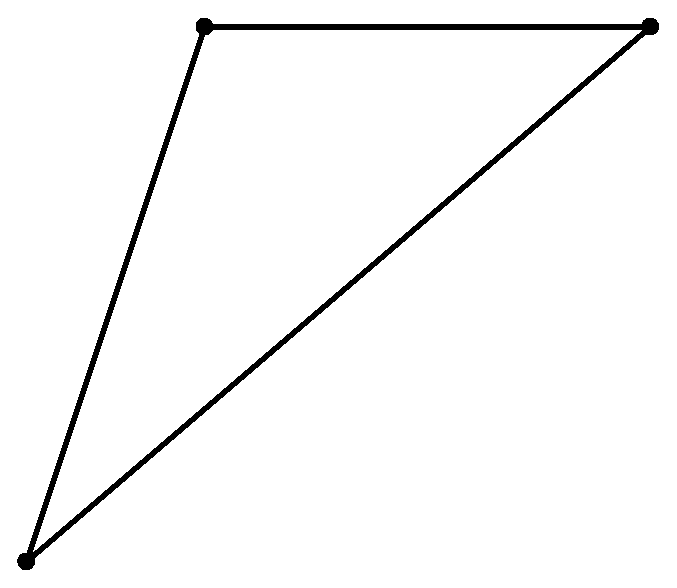
\includegraphics[width=0.35\textwidth]{sketch_triangle}}
        \vspace{0.2in}
        \subfloat[Reference Triangle.]
          {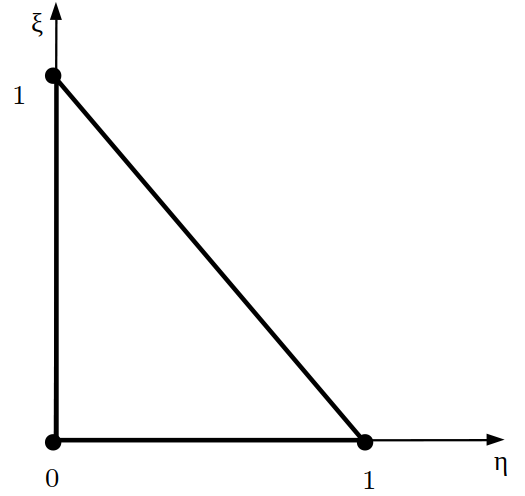
\includegraphics[width=0.35\textwidth]{Tref}}
        \caption{Description of Triangle Elements.}
        \label{fig:triangle_elements}
      \end{figure}

      It is difficult to analytically calculate the desired integral quantities
      for an arbitrary triangle. Instead, a simplified reference element is
      created and quantities are calculated for the reference element and then
      translated to the arbitrary element using a Jacobian. 
      The reference triangle $T_{ref}$ is located in
      $\xi \in [0,1]$ and $\eta \in [0,1-\xi]$. General and reference triangles
      are shown in \fref{fig:triangle_elements}. The
      basis functions are zero outside of the reference triangle and within the
      reference triangle, basis functions for the are provided in the
      coordinates of $T_{ref}$.
      \begin{align}
        \basis_i(\xi,\eta) &= 0 \quad \forall \; (\xi,\eta) \notin T_{ref} \\
        \basis_1(\xi,\eta) &= \xi \\
        \basis_2(\xi,\eta) &= \eta \\
        \basis_3(\xi,\eta) &= 1-\xi-\eta
      \end{align}
      
      The use of reference triangles and Jacobians are general in nature.
      However, for linear triangles there are simple expressions
      for the integral quantities for an arbitrary triangle can be derived
      \cite{textbookwhite}. The expression for
      the line integral for the arbitrary element can also be derived
      \cite{computerLab}. For a triangle with 
      corners $\{ x_i,y_i \}$ with $i=1,2,3$
      \begin{align}
        \int_{\Omega_e} \grad \basis_i(\vr) \cdot \grad \basis_j(\vr) 
          \;d\vr &= \frac{1}{4 A_e}
          ((x_{i+1}-x_{i+2})(x_{j+1}-x_{j+2}) + 
          (y_{i+1}-y_{i+2})(y_{j+1}-y_{j+2})), \\
        \int_{\Omega_e} \basis_i(\vr) \basis_j(\vr) \;d\vr &= 
          \frac{A_e}{12} (1+\delta_{ij}), \\
        \int_{\Omega_e} \basis_i(\vr) \;d\vr &= \frac{A_e}{3}, \\
        \int_{\partial \Omega_e} \basis_i(\vr) \basis_j(\vr) \;ds &=
          \frac{L_e}{6}(1+\delta_{ij}), 
      \end{align}
      where $A_e$ is the area of the triangular element, $L_e$ is the length of 
      the edge between node $i$ and node $j$, and $\delta_{ij}$ is the Kronecker
      delta.
      The Kronecker delta is defined as
      \begin{equation} \label{eq:kroneker_delta}
        \delta_{ij} =
        \begin{cases}
          0 & \text{if } i \ne j, \\
          1 & \text{if } i = j.
        \end{cases}
      \end{equation}
      The area of a triangle in three dimensions is calculated for a triangle
      with corner coordinates $\vc_i = (x_i, y_i, z_i)$ with $i=1,2,3$.
      That is, $\vc_i$ is the coordinates of corner $i$. Calculation of the area
      of a general triangle is then given by the vector operations
      \begin{align}
        \va &= \vc_2 - \vc_1, \\
        \vb &= \vc_3 - \vc_1, \\
        A_e &= \half \lvert \va \times \vc \rvert, \\
        \label{eq:area_triangle}
        A_e &= \half \sqrt{ (a_2 b_3 - a_3 b_2)^2 + (a_3 b_1 - a_1 b_3)^2 +
          (a_1 b_2 - a_2 b_1)^2},
      \end{align}
      where $a_i$ is the $i^{th}$ component of vector $\va$ and $b_i$ is the
      $i^{th}$ component of vector $\vb$.
      For higher order triangular elements, it may be necessary to employ a 
      quadrature to calculate the necessary integral quantities.

    \subsubsection{Linear Wedges}
      A wedge element is a pentahedron with six corner nodes, and is sometimes
      referred to as a triangular prism. A simple example of a wedge is an
      extruded triangle. However, unlike an extruded triangle, the exact 
      geometric relation of corner nodes in a wedge is not fixed and the nodes 
      are free to expand and distort. An example of typical and distorted
      wedge elements are shown in \fref{fig:sketch_wedge}. These elements are
      unique because there are two different types of faces. Three faces are
      quadrilateral and two are triangular. 

      \begin{figure}
        \centering
        \subfloat[General Wedge Element.]
          {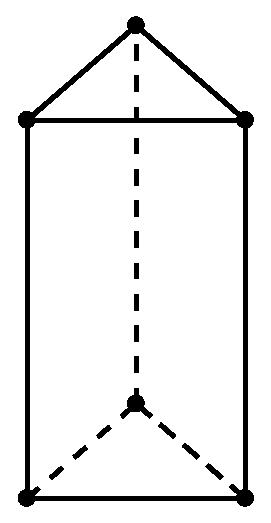
\includegraphics[width=0.2\textwidth]{wedge_sketch}}
        \vspace{0.5in}
        \subfloat[Distorted Wedge Element.]
          {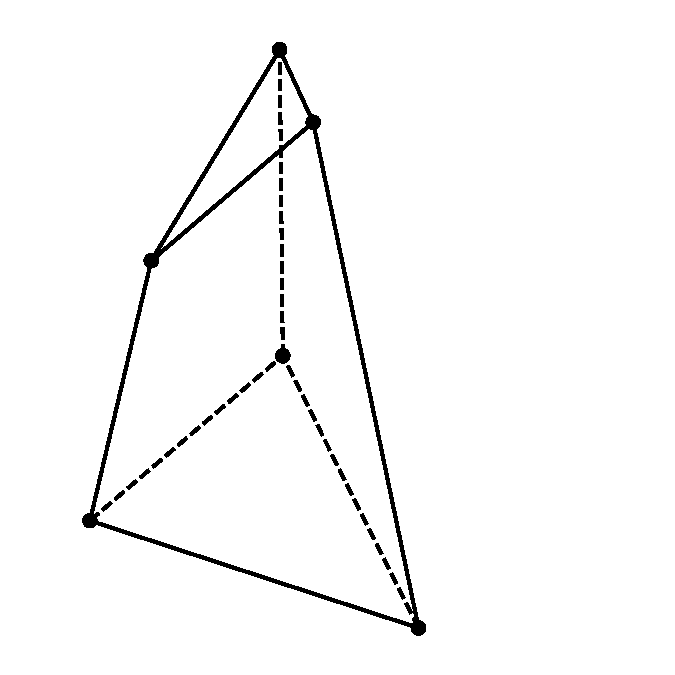
\includegraphics[width=0.2\textwidth]{wedge_stretch}}
        \caption{Description of Wedge Elements.}
        \label{fig:sketch_wedge}
      \end{figure}

      Fast reactors typically have hexagonal-z geometry so wedge elements are a 
      natural choice for this coordinate system. Reactor geometries are also 
      typically described in lattices so the wedge element allows for easily 
      ``stacking'' lattices on top of each other.

      \begin{figure}
        \centering
        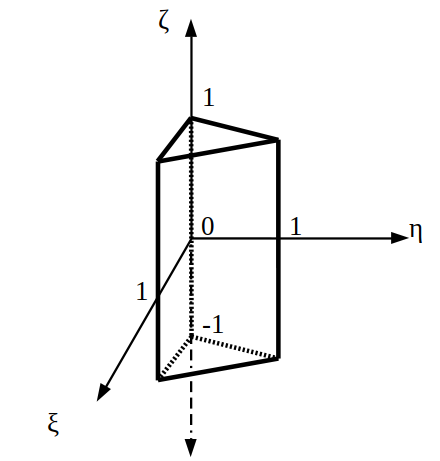
\includegraphics[width=0.3\textwidth]{Wref}
        \caption{Description of Reference Wedge.}
        \label{fig:Wref}
      \end{figure}

      The reference wedge $W_{ref}$ is located in 
      $\xi \in [0,1]$, $\eta \in [0,1-\xi]$, and $\zeta \in [-1,1]$. The
      coordinate system of the reference wedge is shown in \fref{fig:Wref}. The
      basis functions are zero outside of the reference wedge and are 
      provided within the reference wedge.
      \begin{align}
        \basis_i(\xi,\eta,\zeta) &= 0 \quad \forall \; (\xi,\eta,\zeta)
          \notin W_{ref} \\
        \basis_1(\xi,\eta,\zeta) &= \half (1-\zeta)(1-\xi-\eta) \\
        \basis_2(\xi,\eta,\zeta) &= \half (1-\zeta)\xi \\
        \basis_3(\xi,\eta,\zeta) &= \half (1-\zeta)\eta \\
        \basis_4(\xi,\eta,\zeta) &= \half (1+\zeta)(1-\xi-\eta) \\
        \basis_5(\xi,\eta,\zeta) &= \half (1+\zeta)\xi \\
        \basis_6(\xi,\eta,\zeta) &= \half (1+\zeta)\eta 
      \end{align}

      The integrals of the basis function over the element are given in
      \eref{eq:bigmat} through \eref{eq:wedge_surface_integral}. The values
      presented herein are not found in literature and have been calculated by
      the author. For a general wedge, the integral quantities are
      \begin{align}
        \label{eq:bigmat}
        \int_{\Omega_e} \basis_i(\vr) \basis_j(\vr) \;d\vr &= 
          \frac{V_e}{144}
          \begin{pmatrix}
            4 & 2 & 2 & 2 & 1 & 1 \\
            2 & 4 & 2 & 1 & 2 & 1 \\
            2 & 2 & 4 & 1 & 1 & 2 \\
            2 & 1 & 1 & 4 & 2 & 2 \\
            1 & 2 & 1 & 2 & 4 & 2 \\
            1 & 1 & 2 & 2 & 2 & 4 
          \end{pmatrix} \\
        \int_{\Omega_e} \basis_i(\vr) \;d\vr &= \frac{V_e}{12} \\
        \label{eq:wedge_surface_integral}
        \int_{\partial \Omega_e} \basis_i(\vr) 
          \basis_j(\vr) \;ds &= 
          \begin{cases}
            \frac{A_{\Delta}}{12}(1+\delta_{ij})&\text{if triangular surface} \\
            \frac{A_{\Box}}{36}(1+\delta_{ij})(1-\half \delta_{i,(5-j)}) &
              \text{if quadrilateral surface}
          \end{cases}
      \end{align}
      where $V_e$ is the volume of the element, $A_{\Delta}$ is the area of the
      triangular surface, and $A_{\Box}$ is the area of the quadrilateral
      surface. 
      The matrix in \eref{eq:bigmat} is indexed $M_{ij}$
      and is presented as a matrix because of its irregular form. Notice the 
      integral containing the gradient operator has been omitted because it is
      computed using a quadrature. If it could be computed analytically, it 
      would be less computationally efficient than using a quadrature.
      
      $A_{\Delta}$ is computed according to \eref{eq:area_triangle} and
      $A_{\Box}$ is computed as the sum of the area of two triangles, employing
      the same formula. For a simple extruded triangle, the volume calculation 
      is straightforward and is the product of triangular area and linear 
      height. However, allowing the nodes to move with respect to each other 
      makes the volume of the element difficult to calculate. Therefore, the 
      Jacobian is used to calculate $V_e$. For more detail, see 
      \sref{sec:quadratures}, especially \tref{tab:jacobi}.

  \subsection{Quadratures}
    \label{sec:quadratures}
    Quadratures are sets of coordinates and weights which allow for the exact 
    integration of polynomials of given order. For a given set of weights 
    $\{w_i\}$ and a set of coordinates $\{\vx_i\}$, an integral can be 
    represented as the sum
    \begin{equation}
      \label{eq:quadrature}
      \int_{\Omega} f(\vx) \;d\Omega \approx \sum_{i=1}^{N} w_i f(\vx_i)
    \end{equation}
    where $\Omega$ is an arbitrary domain described by $\{\vx_i\}$. The 
    quadratures in \eref{eq:quadrature} will exactly integrate a polynomial of
    the order of the quadrature, $n$. It is not necessarily true that $N$ be the 
    order of the quadrature. Generally, $n \ne N$.
    
    For one-dimensional integrals, the Gaussian quadrature is common and the 
    most compact quadrature. The Gaussian quadrature exactly integrates a 
    polynomial of order $n$ using exactly $n$ points. For this quadrature, the
    number of points in the quadrature is the same as the order of the
    quadrature and $n=N$.
    
    Two-dimensional and three-dimensional quadratures are necessary for the 
    \gls{fem}. Triangular quadratures are not as simple to derive
    as line quadratures and the number of points need not equal the order of the
    polynomial integrated. The triangular quadrature as implemented here is 
    symmetric and open. That is, there are no points on the boundary of the 
    triangle \cite{triangleQuadrature}. Any triangular quadrature will suffice
    that exactly integrates polynomials of a given order. There is no fixed
    relationship between $n$ and $N$ and for this quadrature, $n \ne N$.
    
    Quadrilateral quadrature sets are simply tensor products of two line 
    Gaussian quadratures. For an order $N$ polynomial, now $n^2$ points are 
    required. 
    
    Wedge quadrature sets are simply tensor products of a line Gaussian 
    quadrature and a triangular quadrature. 
    
    Basis functions are polynomials of first, second, or third order. These 
    quadratures are capable of exactly integrating polynomial functions of given
    order so there exists a quadrature order that will exactly integrate the 
    finite element quantities to numeric precision. The table of the order
    required for exact integration are provided in \tref{tab:quadrature_orders}.

    \begin{table}
      \begin{center}
        \caption{Quadrature Orders for \glsentryshort{fem} Quantities.}
        \label{tab:quadrature_orders}
        \begin{threeparttable}
          \begin{tabular}{lccc}
            \toprule
            Quantity & Linear & Quadratic & Cubic \\
            \midrule
            $\int_{\Omega} \basis_i(\vr) \;d\Omega$ & 1 & 2 & 4
              \tnote{$\dagger$} \\
            $\int_{\Omega} \basis_i(\vr) \basis_j(\vr) \;d\Omega$ &
              2 & 4 & 6 \\
            $\int_{\Omega} \grad \basis_i(\vr) \cdot \grad \basis_j(\vr) 
              \;d\Omega$ & 2 & 3 & 5 \\
            \bottomrule
          \end{tabular}
          \begin{tablenotes}
            \item[$\dagger$] A third-order quadrature would be exact but the 
              quadrature would have negative weights so a fourth order 
              quadrature is selected.
          \end{tablenotes}
        \end{threeparttable}
      \end{center}
    \end{table}
    
    All of the quadratures described here are tabulated for a reference element
    be it a line, triangle, quadrilateral, or wedge. Integration in the 
    \gls{fem} is performed on an arbitrary element in space. Therefore, it is 
    necessary to perform a coordinate transform when using a quadrature set.
    % get VERY explicit here so someone else can actually solve the problem...
    Integration with transformed coordinates from domain $\Omega$ to the
    reference domain $\Omega_{ref}$ can be written
    \begin{equation}
      \int_{\Omega} f(\vx) \;d\Omega = 
        \int_{\Omega_{ref}} f(\vx) \lvert \mj \rvert \;d\Omega_{ref} \approx
        \sum_{i=1}^{N} w_i f(\vx_i) \lvert \mj_i \rvert
    \end{equation}
    where $\mj$ is the Jacobian matrix, $\mj_i$ is the Jacobian matrix at 
    quadrature coordinate $\vx_i$, and $\lvert \cdot \rvert$ represents
    the matrix determinant. Notationally, $J=\lvert \mj \rvert$ and is termed
    the Jacobi.

    Isoparametric elements are elements in which shape functions can be used to
    relate global coordinates, $(x,y,z)$, to local coordinates
    $(\xi,\zeta,\eta)$. Generally, non-curved elements are isoparametric. For 
    isoparametric elements such as triangles and wedges, the Jacobi is constant 
    over the element and can be precalculated to avoid populating, and 
    evaluating the determinant of a matrix for each integration point. For the 
    elements of concern, these values are presented in \tref{tab:jacobi} 
    \cite{textbookcolorado}.
    \begin{table}
      \caption{Jacobi for Selected Elements.}
      \label{tab:jacobi}
      \begin{center}
        \begin{tabular}{ll}
          \toprule
          Element & $J$ \\
          \midrule
          Triangle      & $A_e$ \\
          Quadrilateral & $\frac{1}{4} A_e$ \\
          Wedge         & $\half V_e$ \\
          \bottomrule
        \end{tabular}
      \end{center}
    \end{table}

    For the general element, the Jacobian matrix, $\mj_i$, is calculated at each
    point of the quadrature $(\xi_i,\zeta_i,\eta_i)$ as described in
    \eref{eq:calcJacobian}.
    \begin{equation}
      \label{eq:calcJacobian}
      \mj_i = 
      \begin{pmatrix}
        \sum_{k=1}^{N_P} \left. \frac{\partial \basis_k}{\partial \xi}
          \right|_{(\xi_i,\zeta_i,\eta_i)} x_k   \; &
        \sum_{k=1}^{N_P} \left. \frac{\partial \basis_k}{\partial \zeta}
          \right|_{(\xi_i,\zeta_i,\eta_i)} x_k   \; &
        \sum_{k=1}^{N_P} \left. \frac{\partial \basis_k}{\partial \eta} 
          \right|_{(\xi_i,\zeta_i,\eta_i)} x_k   \\
        \sum_{k=1}^{N_P} \left. \frac{\partial \basis_k}{\partial \xi}
          \right|_{(\xi_i,\zeta_i,\eta_i)} y_k   \; &
        \sum_{k=1}^{N_P} \left. \frac{\partial \basis_k}{\partial \zeta} 
          \right|_{(\xi_i,\zeta_i,\eta_i)} y_k   \; &
        \sum_{k=1}^{N_P} \left. \frac{\partial \basis_k}{\partial \eta} 
          \right|_{(\xi_i,\zeta_i,\eta_i)} y_k   \\
        \sum_{k=1}^{N_P} \left. \frac{\partial \basis_k}{\partial \xi}
          \right|_{(\xi_i,\zeta_i,\eta_i)} z_k   \; &
        \sum_{k=1}^{N_P} \left. \frac{\partial \basis_k}{\partial \zeta} 
          \right|_{(\xi_i,\zeta_i,\eta_i)} z_k   \; &
        \sum_{k=1}^{N_P} \left. \frac{\partial \basis_k}{\partial \eta} 
          \right|_{(\xi_i,\zeta_i,\eta_i)} z_k   
      \end{pmatrix}
    \end{equation}
    In \eref{eq:calcJacobian}, $N_P$ is the number of points in the element, 
    $\basis_k(\vr)$ is the basis function centered at the $k^{th}$ corner, and 
    for corner cordinates $(x_k,y_k,z_k)$ for $k = 1,2,\ldots,N_P$.

    With the Jacobian populated as \eref{eq:calcJacobian}, $J=\lvert\mj\rvert$
    is simply the matrix determinant. For the quadrature integration of 
    derivative quantities as necessary in the \gls{fem}, the derivatives must 
    also be translated from the reference element to the spatial element. This 
    is performed according to \algorithmref{algorithm:deriv_int}. The notation 
    is dense as the method requires two sets of coordinates. First, the 
    coordinate in the reference element $(\xi,\zeta,\eta)$ and second, the 
    coordinate in Cartesian space $(x,y,z)$.

    The vector $\vd_{i,\,(\xi,\zeta,\eta)}$ is the gradient vector for
    $\basis_i$ with respect to the reference coordinates $(\xi,\zeta,\eta)$.
    \begin{equation}
      \vd_{i\,(\xi,\zeta,\eta)} = \grad_{(\xi,\zeta,\eta)} N_i(\vr) 
    \end{equation}
    Vector $\vd_{i,\,(x,y,z)}$ is the gradient vector for $\basis_i$ with
    respect to the Cartesian coordinates $(x,y,z)$. 
    \begin{equation}
      \vd_{i,\,(x,y,z)} = \grad_{(x,y,z)} N_i(\vr)
    \end{equation}
    In \algorithmref{algorithm:deriv_int}, the quadrature has points $\{\vx_p\}$ 
    and weights $\{w_p\}$ for $p = 1,2,\ldots,N$ and the value of the integral
    is represented by \eref{eq:deriv_integral}.
    \begin{equation}
      \label{eq:deriv_integral}
      v = \int_{\Omega_e} \grad \basis_i(\vr) \cdot \grad \basis_j(\vr) \;
        d\Omega_e
    \end{equation}

    \begin{algorithm}
      \caption{Integral of Derivative with Jacobian Method.}
      \label{algorithm:deriv_int}
      \begin{algorithmic}[1]
        \State $v=0$
        \For{$p=1,N_P$}
          \State Calculate the Jacobian $\mj$ as in \eref{eq:calcJacobian}.
          \State Calculate the vector $\vd_{i,\,(\xi,\zeta,\eta)}$ at quadrature
            point $\vx_p$.
          \State Calculate the vector $\vd_{j,\,(\xi,\zeta,\eta)}$ at quadrature
            point $\vx_p$.
          \State Invert and store the Jacobian $\mj^{-1}$.
          \State Calculate the vector $\vd_{i,\,(x,y,z)} =
            \vd_{i,\,(\xi,\zeta,\eta)} \mj^{-1}$.
          \State Calculate the vector $\vd_{j,\,(x,y,z)} =
            \vd_{j,\,(\xi,\zeta,\eta)} \mj^{-1}$.
          \State $v = v + \left(\vd_{i,\,(x,y,z)}^{T} \vd_{j,\,(x,y,z)}\right)
            \, w_p \, \lvert \mj \rvert$
        \EndFor
      \end{algorithmic}
    \end{algorithm}

\section{Power Iterations}
  \label{sec:power_iterations}
  The \gls{fem} is used to solve a fixed source problem for a given source
  distribution $q_g(\vr)$. However, for multigroup problems with a fission 
  source, the problem is an eigenvalue problem and the source is not known a 
  priori. For eigenvalue problems, the problem is also not a fixed-source 
  problem and has many solutions. The method of Power Iterations allows 
  eigenvalue problems to be solved iteratively for the fundamental eigenvalue 
  and eigenvector.

  \subsection{Convergence of Power Iteration Method}
    Noting the \gls{fem} equations can be written as matrix form
    \eref{eq:matrix_notation}, the finite diffusion equation can be rewritten as
    shown by Gehin \cite{gehinThesis}.
    \begin{equation}
      \label{eq:gehin_notation}
      \mb(\vPhi,\keff) \vPhi = \frac{1}{\keff} \mm \vPhi
    \end{equation}
    where $\vPhi$ is the vector of the flux containing all energy groups, matrix 
    $\mb$ contains the diffusion, removal, and all scattering terms, and $\mm$ 
    includes all fission generation and operates on $\vPhi$ and $\keff$. $\mb$
    is an S-matrix and its inverse, $\mb^{-1}$, exists and has all positive 
    elements \cite{nakamura}. Therefore, \eref{eq:gehin_notation} can be 
    rewritten as
    \begin{equation}
      \label{eq:gehin_solution}
      \vPhi = \frac{1}{\keff} \mr \vPhi
    \end{equation}
    where
    \begin{equation}
      \label{eq:gehin_r}
      \mr = \mb^{-1} \mm.
    \end{equation}
    Matrix $\mm$ is non-symmetric and is non-negative and $\mb$ is an S-matrix;
    therefore, $\mr$ is a non-symmetric, non-negative matrix.

    In the solution of \eref{eq:multigroup_diffusion}, the largest eigenvalue,
    $\keff$, is desired. The solution can be found using the method of power
    iterations which can be written as 
    \begin{align}
      \label{eq:power_iteration_phi}
      \vPhi^{(s+1)} &= \frac{1}{\keff^{(s)}} \mr \vPhi^{(s)} \\
      \label{eq:power_iteration_eigenvalue}
      \keff^{(s+1)} &= \keff^{(s)} \frac{\vw^{T} \vPhi^{(s+1)}}
        {\vw^{T} \vPhi^{(s)}} \qquad s = 1,2,\ldots,\infty
    \end{align}
    where $s$ is the iteration counter, $\vw$ is a weighting vector and 
    $\vw^{T} \vPhi$ is the vector inner-product. According to the 
    Perron-Frobenius theorem, a matrix with the properties of $\mr$ has a 
    unique, positive eigenvalue, greater in magnitude than the modulus of all 
    other eigenvalues of the matrix. The weighting vector $\vw$ is arbitrary 
    but does affect convergence rate. For this work,
    $\vw = \{\nu \Sigma_f\}$ such that the inner product 
    $\{\nu \Sigma_f\}^T \vPhi$ represents the summation of the fission neutron
    production rate throughout all energy groups and all elements. 
    
    It can then be shown in that the method of power iterations described in 
    \eref{eq:power_iteration_phi} and \eref{eq:power_iteration_eigenvalue}
    converges to the largest eigenvalue, $\keff$, and unique positive 
    eigenvector $\vPhi$ \cite{nakamura}. For notation and enumeration, allow the 
    eigenvalue to be rewritten as
    \begin{equation}
      \label{eq:mu}
      \mu = \frac{1}{\keff}.
    \end{equation}
    The eigenvectors $\vu_n$ and
    corresponding eigenvalues $\mu_n$ of $\mr$ are defined by
    \begin{equation}
      \label{eq:eigen_definition}
      \vu_n = \mu_n \, \mr \, \vu_n
    \end{equation}
    It may be proved that all eigenvalues $\mu$ are real, positive, and 
    distinct. The eigenvalues are then numbered in the sequence:
    \begin{equation}
      \label{eq:eigen_order}
      \mu_0 < \mu_1 < \mu_2 < \cdots < \mu_I
    \end{equation}
    where $I$ is the rank of the problem. The eigenvectors have the 
    orthogonality relations:
    \begin{equation}
      \label{eq:eigen_orthogonality}
      \vu^T_n \vu_m = 0  \qquad \text{for } n \ne m
    \end{equation}
    where $\vu^T \vu$ is the vector inner-product. Assume eigenvectors are
    normalized such that:
    \begin{equation}
      \label{eq:eigen_normalization}
      \vu_n^T \vu_n = 1 \qquad \text{for } n = 1, 2, \ldots, I.
    \end{equation}
    The initial vector $\vPhi^{(0)}$ may be expressed as a projection onto the
    eigenvectors using a linear superposition of eigenvectors.
    \begin{equation}
      \label{eq:eigen_projection}
      \vPhi^{(0)} = \sum_{n=1}^{I} c_n^{(0)} \vu_n
    \end{equation}
    where $c_n^{(0)}$ is a coefficient given by the orthogonality relationship
    from \eref{eq:eigen_orthogonality} such that
    \begin{equation}
      \label{eq:eigen_cn}
      c_n^{(0)} = \vu_n^T \vPhi^{(0)}.
    \end{equation}
    Using this eigenmode projection, \eref{eq:power_iteration_phi} can be
    rewritten as 
    \begin{equation}
      \label{eq:phi_expand_begin}
      \vPhi^{(s+1)} = \mu^{(s)} \, \mu^{(s-1)} \, \mu^{(s-2)} \, 
        \ldots \, \mu^{(0)} \, \mr \phi^{(0)}.
    \end{equation}
    Then, \eref{eq:eigen_projection} can be inserted into
    \eref{eq:phi_expand_begin}.
    \begin{align}
      \vPhi^{(s+1)} &= \mu^{(s)} \, \mu^{(s-1)} \, \ldots \, 
        \mu^{(0)} \sum_{n=1}^I c_n^{(0)} \, \mr \, \vu_n \\
      &= \left( \prod_{p=0}^{s} \mu^{(p)} \right) \sum_{n=1}^I c_n^{(0)} \, 
        \mr \, \vu_n
    \end{align}
    Recalling the relationship \eref{eq:eigen_projection}
    \begin{equation}
      \label{eq:phi_expand_above}
      \vPhi^{(s+1)} = \left( \prod_{p=0}^s \mu^{(p)} \right) 
        \sum_{n=1}^I c_n^{(0)} \frac{1}{\mu_n^{(s+1)}} \vu_n
    \end{equation}
    \eref{eq:phi_expand_above} can be rewritten by dividing and multiplying by
    $\mu_0$ and dividing and multiplying by $c_0$.
    \begin{align}
      \vPhi^{(s+1)} &= \left( \prod_{p=0}^s \frac{\mu^{(p)}}{\mu_0} 
        \right) c_0 \left( \vu_0 \sum_n^I \frac{c_n^{(0)}}{c_0^{(0)}}
        \frac{\mu_0}{\mu_n^{(s+1)}} \vu_n \right) \\
      \label{eq:eigen_phi_converge}
      \vPhi^{(s+1)} &\approx \text{const.} \left( 
        \vu_0 \sum_n^I \frac{c_n^{(0)}}{c_0^{(0)}}
        \frac{\mu_0}{\mu_n^{(s+1)}} \vu_n \right)
    \end{align}
    The ordering of unique eigenvalues required by \eref{eq:eigen_order} 
    requires $\mu_0 / \mu_n < 1$ and the problem is convergent. The 
    convergence rate is determined by the dominance ratio, $d$, where
    \begin{equation}
      \label{eq:dominance_ratio}
      d \equiv \max_{n=1,2,\ldots,I} \frac{\mu_0}{\mu_n} =
        \frac{\mu_0}{\mu_1}
    \end{equation}
    and it can be seen that for problems with small dominance ratio, the power
    iteration method will converge more quickly. As the dominance ratio
    approaches unity, $d \rightarrow 1$, the Power Iteration method will be
    slower to converge. Convergence criteria are then specified as an absolute 
    tolerance in the sense of the eigenvalue
    \begin{equation}
      \label{eq:eigenvalue_tol}
      \epsilon_{\mu} > | \mu^{(s+1)} - \mu^{(s)} |
    \end{equation}
    and as a relative tolerance in the sense of the eigenvector
    \begin{equation}
      \label{eq:eigenvector_tol}
      \epsilon_{\vPhi} > \max_i \left| \frac{\vPhi_i^{(s+1)} - \vPhi_i^{(s)}}
        {\vPhi_i^{(s)}}\right| .
    \end{equation}

    It is important to note that all of the analysis in this section assumed the
    matrix $\mr$ does not change between iterations. For simple multigroup
    criticality calculations, this assumption is correct. However, in realistic
    power reactor simulations, the cross-sections of the problem may be 
    considered functions of material temperature or may have some variable
    number density. For these problems, the matrix $\mr$ is necessarily updated
    between power iterations in a nonlinear manner. For nonlinear power
    iteration updates, convergence is no longer guaranteed. The argument for
    convergence with nonlinear power iterations in this implementation falls 
    back to the stability of the physical system.
    
  \subsection{Calculation of Source with Power Iterations}

    The multigroup neutron diffusion equation \eref{eq:multigroup_source} can be
    written with the source term $q_g(\vr)$ expanded into its component parts.
    \begin{equation} \label{eq:multigroup_source_expand}
      -\grad \cdot (D_g(\vr) \grad \phi_g^{(s)}(\vr)) + \Sigma_{r,g}(\vr)
      \phi_g^{(s)}(\vr) = q_{fiss,g}(\vr) + q_{up,g}(\vr) + q_{down,g}(\vr)
    \end{equation}
    Recall from the definitions of the source components that their calculation
    requires the flux $\phi_g(\vr)$. The source components each require
    different energy groups of the flux distribution to be known. The fission
    component $q_{fiss,g}(\vr)$ requires all groups. The up-scatter component
    $q_{up,g}(\vr)$ requires lower energy groups (i.e. $g' > g$). The
    down-scatter component $q_{down,g}(\vr)$ requires higher energy groups (i.e.
    $g' < g$). Based on these requirements, these source components can be
    calculated based on different iterations within the Power Iteration method.
    This is described in \algorithmref{algorithm:general}.
    \eref{eq:multigroup_source_expand} is then more explicitly written.
    \begin{equation} 
      \label{eq:multigroup_power_iterations}
      -\grad \cdot (D_g(\vr) \grad \phi_g^{(s+1)}(\vr)) + \Sigma_{r,g}(\vr)
      \phi_g^{(s+1)}(\vr) = q_{fiss,g}^{(s)}(\vr) + q_{up,g}^{(s)}(\vr) +
      q_{down,g}^{(s+1)}(\vr)
    \end{equation}

\section{Implementation}
  A \gls{fem} neutron diffusion solution has been developed using 
  the above formulae. The program begins by reading a geometry description 
  specified in a plain text VTK file \cite{vtk}. The VTK format is chosen 
  because it is a standard that can be used with visualization tools such as 
  ParaView \cite{ParaView} and VisIt \cite{VisIt}. Additionally, open-source C 
  and Python packages exist for easy manipulation of the format. Cross sections
  are specified in either a plain text user format or the ISOTXS format as 
  common to fast reactor applications and the multigroup cross-section generator
  \mcc \cite{mcc}. The multigroup neutron diffusion equation is solved according
  to \eref{eq:multigroup_source}. The resulting effective neutron multiplication 
  factor, $\keff$, is written to an output file. The multigroup neutron flux is
  written to a different results VTK file for easy visualization.

  \subsection{Algorithm}
    The algorithm for the solution to the diffusion equation is similar to most
    implementations of the power iteration method to solve the multigroup
    neutron diffusion equation. The algorithm itself is presented in 
    \algorithmref{algorithm:general}. The steps unique to the \gls{fem} are 
    steps \ref{state:fem_matrix} and \ref{state:fem_vector}. These require the 
    quantities previously derived and form the linear system described by the 
    \gls{fem}. 

    In step \ref{state:rcm} the matrix is reordered. Mathematically this has no
    effect on the result as the linear system represented is equivalent. This 
    choice to reorder the system is made to improve computational efficiency. 
    Indexing nodes that are physically proximate with proximate indices causes 
    rows in the finite element matrix $\ma$ to be closely coupled to nearby
    rows. In a general unstructured and unordered mesh rows may be coupled to 
    other random rows in the matrix. This step of reordering the matrix $\ma$ 
    seeks to decrease the bandwidth of the matrix and encourage cache hits when
    accessing coupled values in the linear system. The ordering chosen is the
    \gls{rcm} method and common to sparse linear systems
    \cite{rcm}. An example of the bandwidth reduction provided by the \gls{rcm}
    algorithm is shown in \fref{fig:sparsity_pattern}. The plots show the
    sparsity pattern of the matrix before and after reordering. After
    reordering, the matrix bandwidth is reduced from 2,326 to 81.

    \begin{figure}
      \centering
      \subfloat{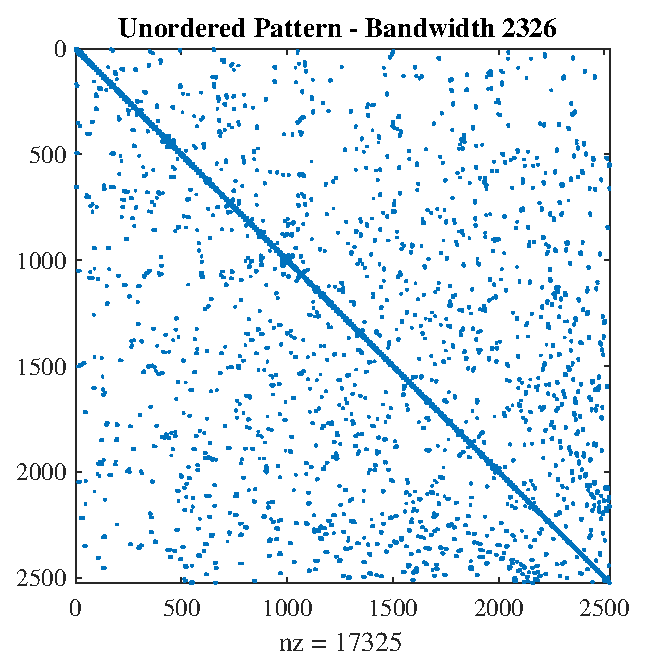
\includegraphics[width=0.4\textwidth]{uno_pattern}}
      \hspace{0.1in}
      \subfloat{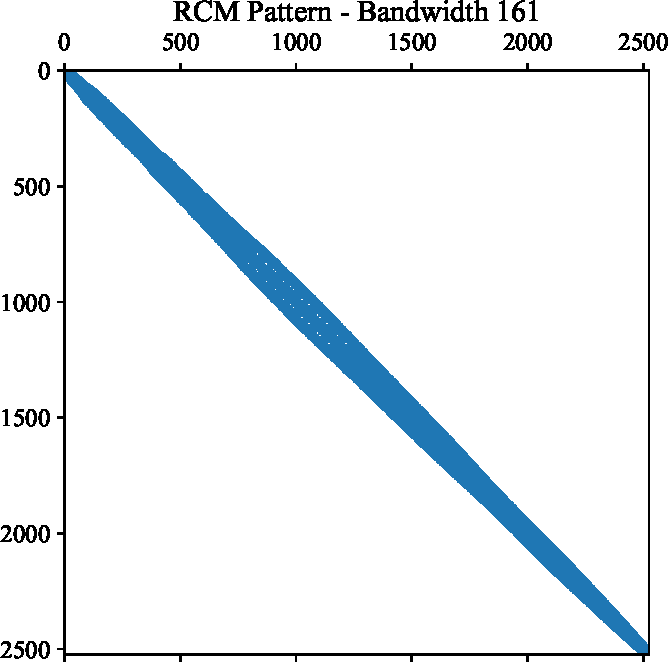
\includegraphics[width=0.4\textwidth]{rcm_pattern}}
      \caption{Demonstration of \glsentryshort{rcm} Matrix Ordering.}
      \label{fig:sparsity_pattern}
    \end{figure}
    
    \begin{algorithm}
      \caption{General Iteration Scheme}
      \label{algorithm:general}
      \begin{algorithmic}[1]
      \State Read mesh from VTK.
      \State Initialize $\phiavg^{(0)}$.
      \State Order the nodes of the mesh into \gls{rcm} order.
        \label{state:rcm}
      \State Calculate $\Sigma_s$, $\Sigma_t$, and $\nu \Sigma_f$ for each 
        element.
      \State Calculate finite element matrix $\ma_g$ for each group. Store this. 
        \label{state:fem_matrix}
      \While{Power Iteration}
        \State Update the iteration counter. $s=s+1$
        \State Update $q_{fiss,g}$ and $q_{up,g}$ for all groups from previous 
          data $\phiavg^{(s-1)}$.
        \State Update $\chi$ in each element using previous data.
          \label{state:chi_collapse}
        \For{$g=1,G$}
          \State Update $q_{down,g}$ from current data $\phiavg^{(s)}$
          \State Calculate total source in each element.
          \State Update finite element Vector $\vf_g$ with new source.
            \label{state:fem_vector}
          \State Solve $\ma \vu = \vf$ using an iterative technique (See
            \sref{sec:linear_system_solution}).
          \State Parse $\vu$ for $\phi$ solution on nodes.
          \State Calculate element-average $\phiavg$.
        \EndFor
        \State Update $\keff$.
        \State Check convergence.
        \State Perform non-linear update if necessary. \label{state:nonlinear}
      \EndWhile
      \end{algorithmic}
    \end{algorithm}

    Step \ref{state:nonlinear} incorporates the possibility of non-linear
    updates into the power iteration method. This invalidates the proof from
    \sref{sec:power_iterations} but is performed to simulate thermal hydraulic
    and thermal expansion effects as described in \chref{ch:thermalHydraulics}
    and \chref{ch:thermalExpansion} respectively. This procedure is commonly
    used in practice and no convergence problems have been observed. This update
    also requires recalculating the finite element matrix $\ma_g$ for each 
    group.
    
    A benefit of this implementation is that the finite element vector $\vf$ 
    must be updated on each power iteration of the solution whereas the matrix 
    $\ma$ is described entirely by geometry and the material cross-sections. For
    this reason, $\ma$ can be generated once at the beginning of the problem and 
    stored for the duration of the calculation (with no non-linear updates).
    \FloatBarrier % make sure the algorithm is in the correct section

  \subsection{Memory and Storage}
    The finite element matrix $\ma$ is large and sparse so a sparse storage and
    sparse solution to the linear system are required. Many sparse matrix 
    implementations have been described and implemented in the past including
    triplet storage, reduced column, and reduced row storage \cite{sparseBLAS}.
    For this work a \twotable method is chosen which was uniquely 
    developed. \twotable storage is chosen for its simplicity and implementation
    with the \gls{fem}. Future work may include a reduced row implementation but 
    there will be a trade-off between memory minimization and computational 
    efficiency.
    
    The \twotable method is composed of two separate matrices in memory. An 
    integer index table, \texttt{IDX}, and an IEEE double precision value table
    \texttt{VAL}. Each table is dimension $DOF \times D$ where $DOF$ is the
    number of degrees of freedom of the linear system and $D$ is the maximum
    number of nodes that a node shares including itself. $D$ is the degree of
    the matrix plus one. This must be determined at the beginning of the
    problem based on the input geometry.
    
    \texttt{IDX} is initialized to -1 and \texttt{VAL} is initialized 
    to 0.0 such that an index of -1 corresponds to a null entry in the 
    matrix. \texttt{IDX} is then populated with a modified adjacency graph. 
    Values in \texttt{IDX} indicate the column in which the \texttt{VAL} entry
    occurs. An example unstructured mesh is given in \fref{fig:adjacency_graph}. 
    Then, for node 5, the table \texttt{IDX} may resemble \eref{eq:idx_example}.
    \begin{equation}
      \label{eq:idx_example}
      \texttt{IDX}(:,5) = (8, 200, 48, 96, 5 )
    \end{equation}
    \begin{figure}
      \centering
      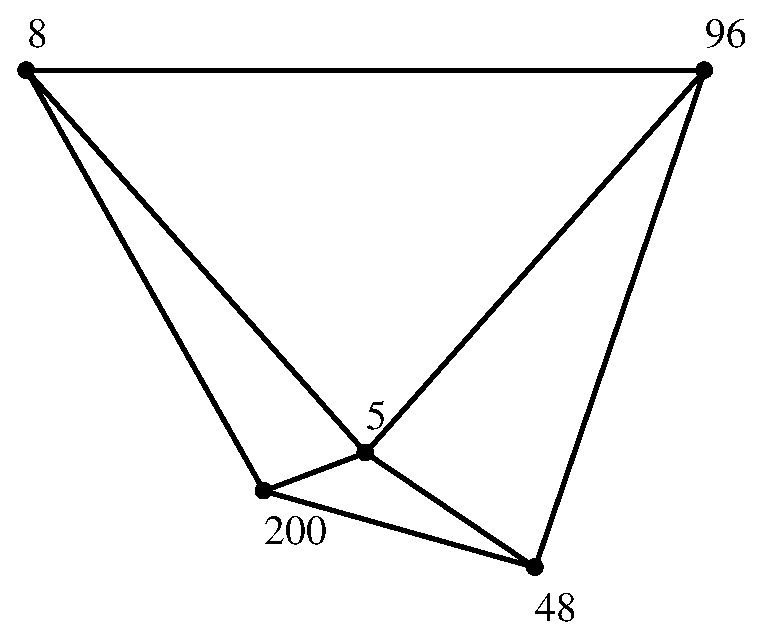
\includegraphics[width=0.5\textwidth]{adjacency_graph}
      \caption{Example Unstructured Mesh.}
      \label{fig:adjacency_graph}
    \end{figure}
    \eref{eq:idx_example} only an example because the order of the nodes in row
    5 is arbitrary. Similarly, a numeric example is provided in 
    \eref{eq:idx_number} (note that the value ``3'' is arbitrary).
    \begin{equation}
      \label{eq:idx_number}
      \left.
      \begin{array}{c}
        \texttt{IDX}(7,3) = 8 \\
        \texttt{VAL}(7,3) = 12.1
      \end{array}
      \right\}
      \implies
      A_{7,8} = 12.1
    \end{equation}
    \eref{eq:idx_number} indicates that the value of matrix $\ma$ in the
    seventh row in the eighth column is 12.1. This will allow for simple row 
    operations and efficient matrix-vector multiplication which will be 
    necessary in the solution of the linear system.

  \subsection{Boundary Conditions}
    \label{sec:boundary_conditions}
    Boundary conditions merit brief consideration. There are many ways to 
    implement boundary conditions and all result in mathematically the same 
    answer. The choices made for this work are presented below. Mirror 
    boundary conditions require $\grad \phi_g(\vr) = 0$ for 
    $\vr \in \partial \Omega$. These are also known as ``natural'' boundary
    conditions because the finite element matrix $\ma$ requires no additional 
    treatment and this condition is natural. In the albedo representation, this
    is equivalent to $\albedo = 0$.
    
    Albedo boundary conditions are treated with an additional contribution to 
    the finite element matrix $\ma$. These contributions represent a line 
    integral in two dimensions and a surface integral in three dimensions. These
    values are found in \eref{eq:matrix_population} and the quantities are 
    expressed in \sref{sec:matrix_quantities} or by quadratures 
    \sref{sec:quadratures}.
    
    Zero-flux boundary conditions require $\phi(\vr) = 0$ for 
    $\vr \in \partial \Omega$. These are treated by removing these entries from
    the finite element matrix $\ma$. Entries are removed by using an index 
    vector. In a natural system (see mirror boundary conditions above) each node
    corresponds to a row/column of the matrix. With entries removed, node number
    and index number may not exactly agree. A vector \texttt{ID} is introduced
    \cite{textbookjohnson}. Nodes with non-zero flux boundary conditions are set
    to a sequential positive integer. Nodes with zero-flux boundary conditions 
    are set to a negative integer (-1) and are omitted in the actual solution of 
    the system. Other strategies have been proposed such as the penalty approach 
    \cite{textbookhughes} and forcing the solution of the linear system 
    \cite{textbookli}. This method is chosen because it decreases the degree of 
    freedom of the linear system while encouraging a well conditioned matrix. 
    Now, the degree of freedom of the matrix is equal to the number of nodes 
    with non-zero flux boundary conditions. Alternatively, zero-flux boundary
    conditions can be represented as $\albedo \rightarrow \infty$.
    
  \subsection{Linear System Solution}
    \label{sec:linear_system_solution}
    For a non-singular linear system $\ma \vu = \vf$, where $\ma$ is a square 
    matrix, there exists a unique solution. Many strategies have been proposed 
    to solve this system in an efficient manner. Options are restricted in this
    work because the solution must operate with a sparsely stored linear 
    system and result in no fill-in. This immediately demands an iterative 
    method. The linear system described by the \gls{fem} can then be exploited 
    for its unique properties to select a favorable solution method.
    
    The finite element matrix $\ma$ for the problem described in 
    \eref{eq:multigroup_source} is \gls{spd} if the
    multigroup equations are solved one group at a time. Note, the matrix will
    not have this especially useful property if all the groups were instead 
    solved simultaneously. Symmetry condition is straight-forward and is 
    observed in the elemental matrix description \eref{eq:matrix_population}. 
    Briefly, ${A_{i,j,g,e}=A_{j,i,g,e}}$.
    Positive definiteness is a particularly useful condition but is often 
    difficult to prove. $\ma$ is sometimes diagonally dominant for conveniently
    ordered meshes composed certain elements but generally, the matrix is not 
    diagonally dominant. 
    
    A matrix $\ma \in \realnn$ is positive definite if
    \begin{equation} \label{eq:positive_definite}
      \vx^{T} \ma \vx > 0 \qquad \forall \vx \in \realn, \; \vx \ne 0
    \end{equation}
    Let $\vx = \{x_i\}$ for $i = 1,2,\ldots,N$. Then the vector-matrix and 
    matrix-vector products can be rewritten as summations \cite{textbookhughes}.
    \begin{equation}
      \vx^{T} \ma \vx = \sum_{i=1}^{N} \sum_{j=1}^{N} x_i A_{ij} x_j
    \end{equation}
    By the definition of $A_{ij}$ in \eref{eq:matrix_population} and 
    \eref{eq:fem_notation}.
    \begin{equation}
      \vx^{T} \ma \vx = 
        \sum_{i=1}^{N} \sum_{j=1}^{N} x_i a(\basis_i,\basis_j) x_j
    \end{equation}
    Noting the property that $a(\cdot,\cdot)$ is a bilinear operator (i.e.
    linear in both arguments) \cite{textbookli}.
    \begin{equation}
      \vx^{T} \ma \vx =
        a \left( \sum_{i=1}^{N} x_i \basis_i, \sum_{j=1}^{N} x_j \basis_j 
        \right)
    \end{equation}
    By construction of the \gls{fem}, $w(\vr) = \sum_{i=1}^{N} x_i \basis_i$ 
    where $w(\vr)$ is a piecewise continuous polynomial of arbitrary order.
    \begin{equation}
      \vx^{T} \ma \vx = a \left(w(\vr),w(\vr)\right)
    \end{equation}
    $a(\cdot,\cdot)$ can be shown to form a norm $\|\cdot \|_a$
    \cite{textbookli} satisfying the positive definite condition
    \eref{eq:positive_definite}.
    \begin{equation}
      \vx^{T} \ma \vx > 0 \qquad \forall \vx \in \realn, \; \vx \ne 0
    \end{equation}
    
    A given matrix can be verified as positive definite by one of two methods.
    First, all eigenvalues of the matrix have positive real components. Second, 
    the matrix has a Cholesky decomposition such that $\ma = \ml \ml^*$ where 
    $\ml$ is a lower triangular matrix with positive diagonal entries and 
    $\ml^*$ is the conjugate transpose of the matrix \cite{textbookipsen}. For 
    real valued matrices, the conjugate transpose is equivalent to the 
    conventional transpose. Though this may be useful for debugging or numerical
    analysis purposes, these operations are computationally expensive. Instead,
    this is verified here for the general matrix and not tested during
    simulations.
    
    Conventional methods used to solve a linear system described by an \gls{spd}
    matrix include Gauss-Seidel iteration with \gls{sor} and the \gls{cg} Krylov 
    subspace method. \gls{sor} needs \textit{a priori} knowledge of the 
    optimized over-relaxation factor $\omega_{opt}$ for optimal performance. In 
    practice, this is performed analytically with contrived solutions or in a 
    modified guess-and-check method. The \gls{cg} method is chosen because it 
    requires no \textit{a priori} knowledge and produced a solution to the same 
    tolerance in a comparable wall-time without the need for guess-and-check 
    iterations.
    
    A simple recipe for the \gls{cg} method is replicated in
    \algorithmref{algorithm:CG} \cite{Kelley1995IterativeEquations}
    
    \begin{algorithm}
      \caption{\glsentrylong{cg} Method.}
      \label{algorithm:CG}
      \begin{algorithmic}[1]
        \State $k = 0$
        \State $\vr = \vb - \ma \vx$
        \State $\rho_k = \|\vr\|_2^2$
        \State $k = k + 1$
        \While{$\sqrt{\rho_{k-1}} > \epsilon \|\vb\|_2$}
          \If{$k=1$}
            \State $\vp = \vr$
          \Else
            \State $\beta = \rho_{k-1} / \rho{k-2}$
            \State $\vp = \vr + \beta \vp$
          \EndIf
          \State $\vw = \ma \vp$
          \State $\beta = \rho_{k-1} / \vp^{T} \vw$
          \State $\vx = \vx + \beta \vp$
          \State $\vr = \vr - \beta \vw$
          \State $\rho_k = \| \vr \|_2^2$
          \State $k=k+1$
        \EndWhile
      \end{algorithmic}
    \end{algorithm}
    
    In \algorithmref{algorithm:CG}, $\epsilon$ is a tolerance set by the user 
    and the square of the two-norm is most efficiently replaced by the vector
    inner-product as in \eref{eq:two_norm_inner}. 
    \begin{equation}
      \label{eq:two_norm_inner}
      \|\vr\|_2^2 = \vr^{T} \vr
    \end{equation}
    It is noted that this method requires minimal storage with only four vectors 
    required ($\vx, \vw, \vp,$ and $\vr$). Additionally, two scalar products 
    are required and a single matrix-vector product which proves to be the most 
    computationally expensive \cite{Kelley1995IterativeEquations}. As most of 
    the computational time of the diffusion solutions is spent in the linear 
    system solution, is is crucial that this process be efficient.

    With the solution of the linear system, the implementation of the \gls{fem}
    to solve the multigroup neutron diffusion problem is completed. Results in 
    the form of analytic and benchmark verification problems are presented in
    \chref{ch:diffusionResults}.
